\chapter{What's a Fair Start?}

In this eighth lecture, Michael Sandel turns explicitly to distributive justice: how income, wealth, power, and opportunity should be distributed, and by what principles. These notes, prepared in the LazyLearn track and curated by LazyingArt LLC, follow the lecture's order closely. We begin with Rawls's contractual setup, move to the two principles of justice, pass through the classroom challenge about merit and effort, and then arrive at the lecture's sharpest distinction, the distinction between moral desert and entitlements to legitimate expectations. The mathematical form of the chapter is schematic rather than economic; its purpose is to display the structure of Sandel's argument without pretending that Rawls's theory is a system of formulas alone.

\section{The Original Position and the First Principle}

Sandel begins by reactivating the machinery prepared in the previous lecture. We are not asked first to admire Rawls's conclusions. We are asked first to enter a device for choosing principles fairly.

\begin{definition}
The \emph{original position} is the hypothetical standpoint from which principles of justice are to be chosen. The \emph{veil of ignorance} specifies the restriction built into that standpoint: we do not know our place in society, our class, our talents, our family background, or our prospects once the veil is lifted.
\end{definition}

The lecture's opening chain can therefore be written schematically as
\begin{equation}
\text{veil of ignorance}
\Longrightarrow
\text{original position of equality}
\Longrightarrow
\text{choice of principles of justice}.
\end{equation}

This order matters. If we know too much about ourselves, we will choose principles that protect our own current advantages. If we know too little, the exercise becomes empty. Rawls's wager is that the veil removes exactly the information that would bias our choice.

\subsection{Question \& Answer}

\paragraph{Question.} Why would parties behind the veil reject utilitarianism?

\paragraph{Answer.} Sandel's answer is practical before it is technical. Once the veil rises, each of us will want to live with dignity, and any of us may turn out to belong to a minority. A principle that maximizes aggregate welfare can permit the sacrifice of some for the happiness of others. That is not a risk rational parties would take when they do not know whether they will be on the winning or losing side.

We can summarize the structure of the rejection in one line:
\begin{equation}
\text{utilitarianism}
\Longrightarrow
\text{possible sacrifice of minorities}
\Longrightarrow
\text{rejected}.
\end{equation}

Sandel then formulates the first principle. The transcript briefly garbles the list of liberties, but the stable content is clear enough:
\begin{equation}
P_1=\text{equal basic liberties}.
\end{equation}

These liberties include freedom of speech, freedom of assembly, religious liberty, freedom of conscience, and related fundamental rights. The priority of this first principle is also crucial. We do not begin with money and only later ask about liberty. We secure the equal liberties first, and only then turn to social and economic inequalities.

\section{From Equal Shares to the Difference Principle}

Once the first principle is in place, Sandel turns to the second question: what should we agree to concerning inequality? Here the lecture is deliberately staged. The first answer is not Rawls's final answer. It is the answer we are likely to give when we feel the force of uncertainty.

If we do not know whether we will be rich or poor, healthy or unhealthy, born into wealth or poverty, then equal shares look initially like the safest rule. Sandel lets that thought appear before he displaces it:
\begin{align}
\text{strict equality} &= \text{equal distribution of income and wealth},\\
\text{strict equality} &\not\Longrightarrow \text{best outcome for the least well-off}.
\end{align}

That second line is the key move. Equal shares are safe, but they may not be best. Rawls's second principle allows us to do better than strict equality, even from the standpoint of those who wind up at the bottom.

\begin{definition}
The \emph{difference principle}, as presented in the lecture, permits social and economic inequalities only when those inequalities work to the benefit of the least well-off.
\end{definition}

In Sandel's lecture notation, we can state the second principle as
\begin{equation}
P_2=\text{allow only those social and economic inequalities that benefit the least well-off}.
\end{equation}

And, in a cautious editorial shorthand that matches the lecture's logic without pretending to reproduce Rawls's own notation, we may write
\begin{equation}
\Delta(\text{income, wealth})>0
\qquad\text{is acceptable only if}\qquad
\Delta(\text{position of the least well-off})>0.
\end{equation}

\subsection{Question \& Answer}

\paragraph{Question.} Why would rational choosers accept some inequality rather than insist on equal shares?

\paragraph{Answer.} Because once we ask not only what is safest but what leaves the worst-off best off, strict equality need not be the optimal rule. An inequality that raises the floor may be preferable to equality that leaves the floor lower. Sandel emphasizes that the test is not whether inequality exists, but whether it improves the condition of those at the bottom.

This is why the familiar salary examples enter so early in the lecture. Michael Jordan's earnings and Bill Gates's fortune are not introduced merely to provoke resentment. They are introduced to sharpen the institutional question: under what kind of scheme, if any, could such inequalities be justified?

\section{Mike, Kate, and the Turn to Moral Arbitrariness}

At this point the lecture becomes overtly dialogical. Sandel asks whether the class accepts Rawls's claim that these two principles would be chosen behind the veil. Mike objects. Why assume that rational choosers would legislate from the standpoint of the disadvantaged? Why not prefer a merit-based system that rewards effort and achievement?

Mike's challenge matters because it presses exactly where the official contract argument seems vulnerable. Perhaps, behind the veil, people would gamble. Perhaps they would take their chances and hope to land near the top.

Sandel's reply is not to abandon the contractual argument, but to supplement it. He says that Rawls has two arguments, not one. The first is the official argument from the original position. The second is a moral argument against basing distributive shares on factors for which people can claim no credit.

Kate's intervention sharpens that second line of thought. She shifts the question from abstract merit to actual social starting points. The lecture gives a striking statistic:
\begin{align}
\text{students from the bottom quarter at selective colleges} &\approx 3\%,\\
\text{students from affluent families} &> 70\%.
\end{align}

The point is not that effort is unreal. The point is that effort takes place inside unequal social conditions. Once this is seen, meritocracy can no longer be treated as self-explanatory.

\subsection{Question \& Answer}

\paragraph{Question.} Why not choose meritocracy behind the veil of ignorance?

\paragraph{Answer.} Because meritocracy seems attractive only if we silently assume that the conditions under which merit is displayed are already fair. Kate's objection is that they are not. Access to good schools, cultural confidence, family support, and economic security enter into achievement long before the competition officially begins. Sandel uses this exchange to widen the argument: the issue is not merely what would be chosen under uncertainty, but whether distributive shares should rest on morally arbitrary contingencies at all.

\section{The Ladder from Aristocracy to the Democratic Conception}

Sandel now reconstructs Rawls's sequence of rival theories. Each step corrects one form of arbitrariness, but each leaves another in place. That rhythm is the backbone of the middle of the lecture.

We can write the ladder of views as a sequence of increasingly demanding criticisms:
\begin{align}
\text{feudal aristocracy} &\Longrightarrow \text{life prospects fixed by accident of birth},\\
\text{formal equality of opportunity} &= \text{careers open to talents},\\
\text{formal equality}+\text{unequal starting points} &\Longrightarrow \text{unfair race},\\
\text{fair equality of opportunity} &\Longrightarrow \text{same starting line},\\
\text{same starting line}+\text{natural lottery} &\not\Longrightarrow \text{full justice}.
\end{align}

\begin{figure}[h]
\centering
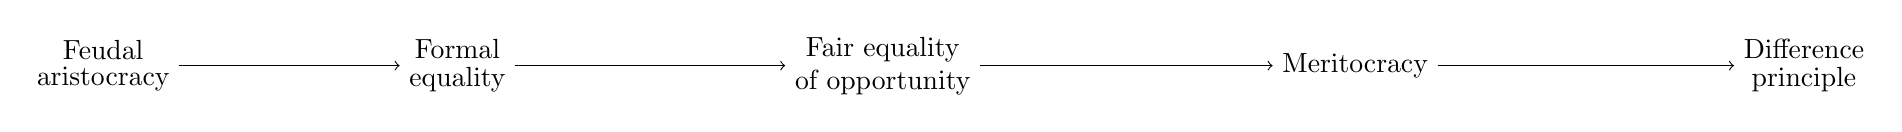
\begin{tikzpicture}[x=3.0cm,y=1.6cm]
\node (a) at (0,0) {\shortstack{Feudal\\aristocracy}};
\node (b) at (1.5,0) {\shortstack{Formal\\equality}};
\node (c) at (3.3,0) {\shortstack{Fair equality\\of opportunity}};
\node (d) at (5.3,0) {\shortstack{Meritocracy}};
\node (e) at (7.2,0) {\shortstack{Difference\\principle}};
\draw[->] (a) -- (b);
\draw[->] (b) -- (c);
\draw[->] (c) -- (d);
\draw[->] (d) -- (e);
\end{tikzpicture}
\end{figure}

The race metaphor organizes the argument. If some runners begin far ahead of others, then merely allowing everyone to run does not make the race fair. That criticism produces fair equality of opportunity, the attempt to bring everyone to the same starting line. But Sandel then asks the next question: if everyone starts together, who wins? The fastest runners. And is it their doing that they have the speed to win?

This is where Rawls goes beyond meritocracy. We are not asked to deny talent. We are not asked to pretend that everyone is equally gifted. We are asked instead whether the benefits flowing from talent should be held unconditionally.

\subsection{Question \& Answer}

\paragraph{Question.} Why are formal equality of opportunity, and even fair equality of opportunity, still not enough?

\paragraph{Answer.} Formal equality leaves family and class advantages intact. Fair equality corrects those social contingencies, but it still leaves untouched the natural lottery. Even after we equalize the starting line, the distribution of native talents continues to determine the winners. If our objection is truly to morally arbitrary influences, Rawls says, then we cannot stop at meritocracy.

Sandel therefore presents the decisive shift in a memorable way. Rawls need not endorse a leveling equality that handicaps the gifted. He can instead alter the terms on which the fruits of talent are held:
\begin{equation}
\text{people may gain from natural good fortune}
\Longrightarrow
\text{only on terms that help the least well-off}.
\end{equation}

\section{Inequality, Pay Differentials, and Incentives}

The lecture now translates principle into institutional judgment. Sandel re-enters the argument through concrete salaries, because the difference principle is not a taste for equality in the abstract; it is a test applied to actual structures of reward.

\paragraph{Worked example.} Consider Sandel's comparison between an ordinary teacher and David Letterman:
\begin{align}
\text{school teacher salary} &\approx \$42{,}000,\\
\text{David Letterman salary} &\approx \$31{,}000{,}000.
\end{align}

Rawls's question is not simply whether the difference is large. It is whether the basic structure of society is arranged so that the higher earnings are partly channeled, through taxation and institutions, to the advantage of those at the bottom.

The worked test runs as follows:
\begin{enumerate}
\item Observe an inequality in rewards.
\item Ask whether the institutional scheme preserves equal liberties.
\item Ask whether the higher return is necessary or useful in a way that improves the condition of the least well-off.
\item If the answer is yes, the inequality may be just under \(P_2\).
\item If the answer is no, the inequality is not justified simply by being produced by the market.
\end{enumerate}

Sandel repeats the point with another comparison:
\begin{align}
\text{Supreme Court justice salary} &< \$200{,}000,\\
\text{Judge Judy salary} &\approx \$25{,}000{,}000.
\end{align}

Again, the lecture refuses the easy conclusion. We are not told that such a differential is automatically unjust. We are told to ask what institutional arrangement surrounds it.

\subsection{Question \& Answer}

\paragraph{Question.} Can the difference principle allow incentives without collapsing into laissez-faire?

\paragraph{Answer.} Yes. This is one of the most careful moments in the lecture. Tim's response, endorsed by Sandel, is that incentives matter, but they must be judged from the right standpoint. The issue is not the total size of the economic pie taken in the abstract. The issue is the effect of incentives and disincentives on the well-being of those at the bottom.

That distinction can be written compactly as
\begin{equation}
\text{incentives judged from standpoint of the least well-off}
\neq
\text{incentives judged by total output alone}.
\end{equation}

This allows Sandel to answer the familiar objection. If very high tax rates would truly reduce productive activity in a way that harms the least well-off, then Rawls can allow a lower tax rate. Incentives are therefore not a decisive objection. They are built into the correct application of the difference principle.

\section{Self-Ownership and the Libertarian Objection}

Sandel next turns to a deeper challenge. The problem is no longer efficiency but ownership. If our talents are ours, why should society tax the gains that flow from them?

He first dismisses an easier libertarian argument associated with Milton Friedman. That argument says that life is unfair, and any attempt to correct nature must result in a disastrous leveling equality of outcome. Sandel replies on Rawls's behalf that this is a false dilemma. Rawls need not equalize outcomes. He asks instead what institutions should do with naturally unequal endowments.

The central Rawlsian line is one of the lecture's most important:
\begin{equation}
\text{natural distribution of talents is neither just nor unjust}.
\end{equation}
What follows from this is equally important:
\begin{equation}
\text{justice}=\text{how institutions deal with those facts}.
\end{equation}

\subsection{Question \& Answer}

\paragraph{Question.} If talents are mine, why may society tax the gains that flow from them?

\paragraph{Answer.} Sandel's answer is careful. Rawls does not deny the person. He does not turn the state into the owner of our lives. The first principle still secures basic liberties. What Rawls denies is the stronger claim that self-ownership yields an unlimited moral title to all market returns generated by our talents. Those returns depend not only on our abilities but on social institutions and on the demand structure of the society in which those abilities are rewarded.

So the dispute is not whether the state may simply commandeer persons. It is whether we have a privileged moral claim to whatever the market happens to pay us. Rawls's answer is that we do not. A just society can protect liberty without treating market reward as the measure of what we deserve.

\section{Effort, Contribution, Desert, and Opportunity}

The final movement of the lecture begins with the meritocratic objection from effort. Surely, one might say, people who work hard to develop their talents deserve what they earn.

Sandel gives Rawls two replies. First, even effort is not simply self-authored. Work ethic, conscientious striving, and ambition are shaped by family background, social circumstances, and, in the lecture's provocative example, even birth order. If effort is partly contingent, then effort alone cannot serve as a clean foundation for distributive shares.

Second, defenders of meritocracy do not in fact reward effort as such. Sandel's construction-worker example makes the point vividly.

\paragraph{Worked example.} Suppose two workers complete the same task:
\begin{align}
\text{Worker A: }& 4\ \text{walls in}\ 1\ \text{hour},\\
\text{Worker B: }& 4\ \text{walls in}\ 3\ \text{days}.
\end{align}

No serious defender of meritocracy would pay Worker B more simply because the task required greater exertion. The operative standard is not sheer effort but contribution. Yet contribution returns us to talent, and talent returns us to the natural lottery.

This is why the lecture culminates in a sharper distinction:
\begin{equation}
\text{moral desert}\neq\text{entitlements to legitimate expectations}.
\end{equation}

Sandel slows down here, and so should we. He distinguishes a game of chance from a game of skill:
\begin{align}
\text{lottery} &\Longrightarrow \text{entitlement without desert},\\
\text{game of skill} &\Longrightarrow \text{entitlement plus a further desert question}.
\end{align}

If our lottery number comes up, we are entitled to the winnings under the rules, but we do not morally deserve to win in any antecedent sense. If a team wins the World Series, it is entitled to the trophy, but we can still ask whether it deserved to win. Rawls's claim is that distributive justice belongs to the first register, not the second: it is about what just institutions entitle us to expect, not about measuring intrinsic worth.

That is why market reward cannot be translated directly into deservingness:
\begin{equation}
\text{supply and demand}\not\Longrightarrow \text{moral desert}.
\end{equation}

What society prizes is contingent. In one society entrepreneurial drive may be richly rewarded; in another, television presence; in another, legal aptitude. The value of those traits in the market is not the same thing as the moral worth of the people who possess them.

\subsection{Question \& Answer}

\paragraph{Question.} Is distributive justice about moral desert, or only about what institutions entitle us to expect?

\paragraph{Answer.} Sandel's answer on Rawls's behalf is that distributive justice is not about moral desert. It is about legitimate expectations under just institutions. We may be entitled to benefits that the rules assign us, but it is a mistake to infer that we therefore deserve, in some prior moral sense, the social order that happens to prize the talents we possess.

This final distinction lets Sandel extend the entire lecture from income and wealth to honors and access. The move is decisive:
\begin{equation}
\text{claims to elite educational opportunity}
\Longrightarrow
\text{subject to the same Rawlsian test as claims to income}.
\end{equation}

\subsection{Question \& Answer}

\paragraph{Question.} Are elite educational opportunities rewards for desert, or entitlements that require public justification?

\paragraph{Answer.} Sandel refuses to settle the admissions question in this lecture, but he states the Rawlsian test clearly. Seats at elite universities should not simply be treated as honors bestowed on those who deserve them because they worked hard. They are also social opportunities, and their justification depends on whether the institutional scheme that distributes them can be defended from the standpoint of those who are least advantaged. The same question we asked of Michael Jordan, David Letterman, and Judge Judy must now be asked of Harvard and other elite institutions.

\section{Summary}

The lecture proceeds in a strict order, and the order is part of the argument. We begin behind the veil of ignorance, reject utilitarianism, and secure the first principle of equal basic liberties. We then pass from strict equality to the difference principle, which allows inequalities only when they improve the condition of the least well-off. From there Sandel pushes beyond the official contract argument to the deeper claim that distributive shares should not rest on morally arbitrary contingencies, whether social or natural. That line of thought carries him past formal equality, past fair equality of opportunity, and past meritocracy itself.

The objections then sharpen the theory. Incentives can be accommodated, but only from the standpoint of those at the bottom. The natural distribution of talents is neither just nor unjust; what matters is the institutional response to it. Effort matters, but it does not rescue moral desert as the basis of distributive justice. In the end the lecture leaves us with Rawls's hardest distinction: not desert, but entitlement under just institutions. And with that distinction in hand, Sandel turns the whole argument toward the next live question, the question of admissions and affirmative action.